\documentclass[10pt, oneside]{article}
\usepackage[utf8]{inputenc}
\usepackage{graphicx} % Required for inserting images
\usepackage{amsmath}
\usepackage{amssymb}
\usepackage[a4paper,left=2.1cm, right=2.1cm, top=2cm, bottom=2cm]{geometry}
\usepackage{verbatim}
\usepackage[english]{babel}
\usepackage{hyperref}
\usepackage{listings}
\usepackage{comment}
\renewcommand{\rmdefault}{cmss}

\lstdefinestyle{mystyle}{	basicstyle=\ttfamily\footnotesize
}

\lstset{style=mystyle}

\title{ROOT}
\author{Pocket reference for 1st year course - BSc Physics, Unibo}
\date{2023}

\begin{document}

\maketitle

\tableofcontents

\section{General structure}

ROOT contains \textbf{interpreter} : \textit{Just-In-Time} compilation $\rightarrow$ prompt : special commands (not standard C++ syntax) with \boxed{\texttt{.}}.

Base class \texttt{TObject} $\rightarrow$ \texttt{TNamed} $\rightarrow$ \texttt{TH1} (histograms) $\rightarrow$ \texttt{TH1F, TH1D, THIC, TH1S} according to \textbf{type representing entries} (not the type of data!!)

\section{Basic shell \& prompt commands}
! Possible to use \boxed{Tab}
\begin{itemize}
\item \boxed{\texttt{root}} launch ROOT
\item \boxed{\texttt{.q}} quit
\item \boxed{\texttt{.L <file.C>}} load file (symbols defined in a macro)
\item \boxed{\texttt{.help}} \boxed{\texttt{.?}} full help list
\item \boxed{\texttt{.! <cmd>}} call any shell command <cmd> without leaving ROOT
\item \boxed{\texttt{.files}} shows loaded libraries / sources
\item \boxed{\texttt{.x <macro>}} loads \& runs a macro
\item \boxed{\texttt{.U <file.C>}} unload
\end{itemize}
Run a macro:
\begin{verbatim}
$ [0] .L <name>.C
$ [1] <name>()
\end{verbatim}
Possible to type C++ commands directly in shell: \textbf{';' are unnecessary, object type can be omitted in declarations, possible to access members with obj name instead than pointer}:
\begin{verbatim}
$ [...] TH1F *histo=new TH1F(“histname”,” Titolo”, 100, 0, 10)
$ histname->Draw() // identical to histo->Draw()
\end{verbatim}
\textbf{Note:} \texttt{\#include <iostream>} and \texttt{namespace std;} are implicit!
\paragraph{Use prompt as calculator}
Ordinary operations + embedded library \texttt{TMath}:
\\\texttt{TMath::Abs(...), TMath::Exp(...), TMath::Gaus(...), TMath::Pi(), ...}
\subsection{Recover session history}
Saved in \texttt{\$/home/.root\_hist}

\section{Histograms}
\textbf{1D}
\begin{verbatim}
TH1F* <pt-name> = new TH1F( "<name>", "<title>", <NxBins>, <xmin>, <xmax>);
// declare new histogram
// range [xmin, xmax] is equally subdivided in N bins

<pt-name>->Fill(<x>); 
// fill histo with variable <x> (e.g. from MC generation or read file, data)

<pt-name>->Fill(<x>, <n>);
// fill histo with n identical occurrences of x

<pt-name>->Draw(); // draw histo
\end{verbatim}
\textbf{2D}
\begin{verbatim}
TH2F* <pt-name> = new TH2F( "<name>","<title>",<NxB>,<xmin>,<xmax>,<NyB>,<ymin>,<ymax>);

<pt-name>->Fill(x,y);
<pt-name>->Draw();

<pt-name>->ProjectionX(); // returns TH1F of projection w.r.t. x
<pt-name>->ProjectionY();
\end{verbatim}
\textbf{3D}
\begin{verbatim}
TH3F* <pt-name> = new TH2F( "<name>","<title>",<Nx>,<xmn>,<xmx>,<Ny>,<ymn>,<ymx>,<Nz>,<zmn>,<zmx>);
\end{verbatim}
\textbf{N-D}
\begin{verbatim}
THnSparse* pt = new THSparse( "<name>", "<title>", <Ndims>, <xmin>, <xmax>, <chuncksize>); 
// min and max same for all dimensions
\end{verbatim}

\subsection{Overlap graphs}
\begin{verbatim}
// declare and initialize two histos, with pointers h1, h2
h1->Draw();
h2->Draw("same"); // or h2->Draw("SameHist");
\end{verbatim}

\subsection{Fit a distribution on a histo}
\begin{verbatim}
h1->Fit("gaus"); // gaussian fit for 1D histo
\end{verbatim}

\subsection{Draw options}
\begin{description}
\item[\texttt{"E"}] show error bars
\item[\texttt{"hist"}] show only histogram
\item[\texttt{"lego"}] lego plot
\item[\texttt{"cont"}] contour lines (linee di livello)
\item[\texttt{"Surf"}] surface
\item[\texttt{"P"}] draw marker (except empty bins)
\item[\texttt{"AXIS"}] draw only axis
\item[\texttt{"AXIG"}] draw only grid (if requested)
\item[\texttt{"FUNC"}]	When histo has fitted function, draw the fit result only.
\item[\texttt{"TEXT"}]	Draw bin contents as text (format set via 
\texttt{gStyle->SetPaintTextFormat}).
\item[\texttt{"X+"}]	The X-axis is drawn on the top side of the plot.
\item[\texttt{"Y+"}]	The Y-axis is drawn on the right side of the plot.
\item[\texttt{"MIN0"}] Set minimum value for the Y axis to $0$, equivalent to \texttt{gStyle->SetHistMinimumZero()}.
\end{description}

\boxed{\textbf{OPTIONS ARE NOT CASE SENSITIVE}}
\\They can also be concatenated without spaces \& commas: \texttt{"opt1 opt2"}
\texttt{h1->SetMarkerStyle(<code>);} set style, see below for codes:
\begin{figure}
\centering
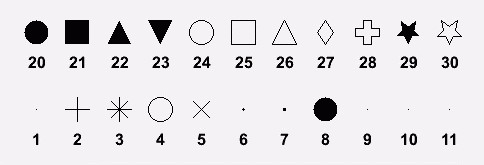
\includegraphics[scale=0.6]{shape.jpg}
\end{figure}
Also \texttt{SetFillColor(...)}, \texttt{SetLineStyle(...)}. \texttt{SetLineColor(...)} avaiable

\subsection{Other member functions for histos}
\begin{description}
\item[\texttt{GetMean()}] mean
\item[\texttt{GerRMS()} \texttt{GetStdDev()}]root of variance / SD
\item[\texttt{GetMaximum()}] maximum bin content
\item[\texttt{GetMaximumBin()}] location of maximum ($\neq$ former)
\item[\texttt{GetBinCenter( <bin\_number> )}] center of bin
\item[\texttt{GetBinContent( <bin\_number> )}] content of bin
\item[\texttt{GetBinError( <bin\_number> )}]
\item[\texttt{SetBinContent( <bin\_number>, <value> )}]
\item[\texttt{SetBinError( <bin\_number>, <value> )}]
\end{description}
\textbf{Note:} for out-of-range entries:
\\\texttt{GetBinContent(0)} returns number of \textbf{underflow}
\\\texttt{GetBinContent(<Nbins + 1>)} return number of \textbf{overflow}
\begin{description}
\item[\texttt{GetEntries()}] total entries (includes under/overflows)
\item[\texttt{Integral( <bin\_index1>, <bin\_index2> )}] integral on specified range
\item[\texttt{Integral()}] total integral
\item[\texttt{GetIntegral()}] array of cumulative entries
\item[\texttt{GetMeanError()}] error on mean estimate
\item[\texttt{GetRMSError()} \texttt{GetStdDevError()}] error on RMS estimate
\end{description}

\subsection{Operations on histos}
Form homologue histograms (\textbf{same range and number of bins}): overloads for \textbf{istances}, \textbf{NOT POINTERS}:
\begin{verbatim}
TH1F h1;
TH1F h2 = 3*h1;
TH1F h3 = h1+h2;
\end{verbatim}
Otherwise through methods:
\begin{verbatim}
h->Add(<pt1>, <pt2>, <n1>, <n2>); // sum stored in *h, *h = n1*h1+n2*h2
h->Multiply(3);
h->Divide(<pt1>, <pt2>, <n1>, <n2>); // analogous to sum
\end{verbatim}

\section{Macros}
Two types of script
\paragraph{Unnamed script} all code between \{\} + no declaration of classes, functions + no parameters (ok loops)
\paragraph{Named script} like any C++ function + possible to define other functions, classes, use parameters
\\The executed function has the same name of the file (see Basics)

\section{GUI}
\boxed{\texttt{TBrowser b}} opens root files browser. 
\\Double click on an object (e.g. histo) $\rightarrow$ opens new \textbf{TCanvas} and draws it
\paragraph{Handling TCanvas}
(if some of the followings not visible, click \textbf{View} and check out
\begin{description}
\item[Editor] single left click on an object in graph $\rightarrow$ edit display parameters (color etc.)
\item[Toolbar] tools to insert text, symbols, etc.
\item[Status bar] shows object pointed by mouse \& mouse position
\item Right click on object $\rightarrow$ contextual menu
\end{description}
\paragraph{Contextual menu}
\begin{description}
\item[Rebin] redefine binning
\item[Fit (of FitPanel)] fit a function on data (gaussian, exponential, polynomial etc.) $\rightarrow$ button \texttt{Set Parameters} for chosen distribution
\end{description}
To visualize fit on graph: right click on graph $\rightarrow$ open \texttt{TPaveStats::stats} $\rightarrow$ \texttt{SetOptFit} $\rightarrow$ se to \texttt{111}
\\\texttt{SetOptStat} allows do define other options
\paragraph{Canvas options} Right click on canvas $\rightarrow$ \texttt{SetLogx}, \texttt{SetLogy} for logarithmic scale; \texttt{SetGridx}, \texttt{SetGridy} for grid
\paragraph{Saving file} \texttt{File} $\blacktriangleright$ \texttt{Save} (\texttt{Save As})
\\Saving as \texttt{.C} file (containing the graph as C++ commands) enables to reproduce graph executing macro
\\Saving as \texttt{.root} file $\rightarrow$ saves canvas and all objects, double click on canvas inside .root (opened through TBrowser) to open and manipulate graph

\section{Global variables}
\begin{description}
\item[\texttt{gROOT}] global info on current session: access to \textbf{every object created during session}
\item[\texttt{gFile}] current root file
\item[\texttt{gStyle}] access functionalities to manage graphic style
\item[\texttt{gRandom}] access random number generator (see MC)
\end{description}
\paragraph{Suggestion} at the beginning of a macro, to eliminate copy created by multiple executions of code in a session:
\begin{verbatim}
delete gROOT->FindObject("<name>");
\end{verbatim}
(\texttt{FindObject("<name>")} used to retrieve every object from gROOT

\section{Managing .root files}
\begin{description}
\item[\texttt{TFile *file = new TFile("<name>.root", "RECREATE");}] open file. \texttt{RECREATE} creates new file if name not found, otherwise overwrites existing one. Alternative option: \texttt{"NEW"} (error if already existing!)
\item[\texttt{h->Write();}] write object (pointed by \texttt{h}) on file
\item[\texttt{file->Close();}] close
\end{description}

\section{Graphs}
Two classes: \textbf{\texttt{TGraph}} (series of N X-Y couples), \textbf{\texttt{TGraphErrors}} (derived from former, includes also errors on both X and Y)
\paragraph{TGraph Constructors}
\begin{description}
\item[\texttt{TGraph (Int\_t n, const Double\_t *x, const Double\_t *y)
}] n couples, \texttt{x} and \texttt{y} are \textbf{arrays}!
\item[\texttt{TGraph (const char *filename, const char *format="\%lg \%lg", 
Option\_t *option="")}] input file \textbf{must contain 2 separate columns of values} (divided by blank delimiter) 
\\Default format: \texttt{"\%lg \%lg"} (2 double), to skip columns: \texttt{\%lg \%*lg \%lg"}
\\Additional options to interpret different delimiters: can be explicitly specified in option argument ( \texttt{option = "<symbol>"} )
\end{description}
\paragraph{TGraphErrors Constructors}
\begin{description}
\item[\texttt{TGraphErrors (Int\_t n, const Double\_t *x, const Double\_t *y, const Double\_t*ex=0, const Double\_t *ey=0)}] analogous to TGraph, \texttt{ex}, \texttt{ey} = arrays of errors
\item[\texttt{TGraphErrors (const char *filename, const char *format="\%lg \%lg \%lg \%lg", Option\_t *option="")}] input file \textbf{must contain at least 3 columns}. If there are 4 (or more, only first 4 read): X, Y, EX, EY. If only 3: X,Y,EY.
\end{description}
\boxed{\textbf{COMMA FOR DECIMALS MUST BE REPLACED WITH DOT}}

\subsection{Graph member functions}
(\texttt{graph} here is the pointer)
Cosmetics:
\begin{description}
\item[\texttt{graph->SetTitle("<title>")}]
\item[\texttt{graph->SetMarkerStyle(kOpenCircle}] (here \texttt{kOpenCircle} is default code)
\item[\texttt{graph->SetMarkerColor(kBlue)}] (\texttt{kBlue} also default)
\item[\texttt{graph->SetLineColor(kBlue)}] ...
\end{description}
Statistical properties:
\begin{description}
\item[\texttt{graph->GetCorrelationFactor()}]
\item[\texttt{graph->GetCovariance()}]
\item[\texttt{graph->GetPoint(<i>,<x>,<y>)}] returns \texttt{i}-th point
\item[\texttt{graph->GetX() / graph->GetY()}] returns pointer to array of x / y values
\item[\texttt{graph->GetN}]
\item[\texttt{graph->Integral()}]
\item[\texttt{graph->AddPoint(<x>,<y>)}]
\item[\texttt{graph->SetPoint(<i>, <x>, <y>)}]
\end{description}

\subsection{Drawing graphs}
\begin{description}
\item[\texttt{graph->Draw(<options>)}]
\item[\texttt{"A"}] draws axes
\item[\texttt{"P"}] draws points markers
\item[\texttt{"E"}] draws error bars
\end{description}

\subsection{Fit}
\begin{description}
\item[\texttt{graph->Fit( <string> )}] \texttt{<string>} contains C++ expression
\item[\texttt{graph->Fit( TF1* f1 }] with previously defined function (see after)
\item[\texttt{TF1* fitFunc = h->GetFunction("f1")}] recover fit function from histo (analogous for graph)
\item[\texttt{fitFunc->GetChiSquare()}]
\item[\texttt{fitFunc->GetParameter(<i>)}] \texttt{i}-th parameter value
\item[\texttt{fitFunc->GetParError(<i>)}] error on \texttt{i}-th parameter
\end{description}

\subsubsection{Statistics \& fit parameters}
\texttt{gStyle->SetOptStat(<ksiourmen>)} choose which statistics param. to display (each mode with a value - default if omitted): k (kurtosis), s (skewness), i (integral), o (overflows), u (underflows), r (1 rms, 2 +rms error), m (1 mean, 2  +mean error), e (entries), n (name) 
\\\texttt{gStyle->SetOptFit(<pcev>)} analogous for fit parameters: p (probability), c (chisquare / dof), e (errors), v (name/value of params: 1 only non-fixed, 2 all)

\section{Functions}
In 1 variable (x): class \textbf{TF1}. User-defined function (and function objects, lambda) or built-in function objects $\rightarrow$ \textbf{TFormula}
\\For more dimensions (variables) \textbf{TF2, TF3}.
\begin{description}
\item[\texttt{TF1 *f1 = new TF1("f1", "sin(x)/x“,<xmin>,<xmax>)}]
\item[\texttt{TF1 *f2 = new TF1("f2", "f1 * 2",0,10)}] previously defined functions can be used in definition of new ones
\item[\texttt{TF1 *f3 = new TF1("f3","[0]*x*sin([1]*x)",-3,3)}] possible to use parameters: to \textbf{initialize} them, \\\texttt{f3->SetParameter(<value0>, <value1>)}
\end{description}
\begin{lstlisting}[language=C++]
Double_t MyFunction(Double_t *x, Double_t *par){ 
	Float_t xx = x[0];
	Double_t val = TMath::Abs(par[0]*sin(par[1]*xx)/xx); 
	return val;
}
\end{lstlisting}
\textbf{Note:} important to follow this signature!
\begin{description}
\item[\texttt{TF1 *f4 = new TF1("f4",MyFunction,0,10,2);}] last constructor parameter is \textbf{number of parameters in MyFunction}
\end{description}
Cosmetics
\begin{description}
\item[\texttt{f1->SetLineColor(kRed)}]
\item[\texttt{f1->SetLineStyle(2)}] 2 = dashed, 3 = dotted, 4 = dasheddotted
\end{description}
Member functions:
\begin{description}
\item[\texttt{f1->Eval(<x\_value>)}] evaluate on a point
\item[\texttt{f1->Integral(<a>, <b>)}]
\end{description}

\section{Legend}
\begin{verbatim}
TLegend *leg = new TLegend(.1,.7,.3,.9,“ <title> "); 
leg->AddEntry(graph,"Punti sperimentali"); 
leg->AddEntry(f,“Fit Lineare"); 
leg->Draw("Same"); 
\end{verbatim}

\section{Canvas syntax}
\texttt{myCanvas->Print("<image-file>")}










\end{document}